\documentclass{classrep}
\usepackage[utf8]{inputenc}
\usepackage[pdftex]{graphicx}
\usepackage[polish]{babel}
\usepackage{algorithm}
\usepackage{algorithmic}
\usepackage{multicol}
\usepackage{amsmath}
\usepackage{listings}
\usepackage{array}
\usepackage{multirow}
\usepackage{url}
\usepackage{subfigure}
\usepackage{hyperref}

\studycycle{Informatyka, studia dzienne, II st.}
\coursesemester{I}

\coursename{Przetwarzanie obrazów i dźwięków}
\courseyear{2010/2011}

\courseteacher{dr inż. Bartłomiej Stasiak}
\coursegroup{micmic}
\svnurl{https://serce.ics.p.lodz.pl/svn/labs/poid/bsat_wt1415/micmic}

\author{%
  \studentinfo{Michał Janiszewski}{169485} \and
  \studentinfo{Michał Kawski}{169487}
}

\title{Zadanie 2: Filtracja w dziedzinie częstotliwości}

\floatname{algorithm}{Algorytm}

\begin{document}

\maketitle

\section{Cel zadania}
Celem zadania było rozwinięcie aplikacji powstałej w wyniku wykonania zadania 1. o możliwości filtrowania obrazów w dziedzinie częstotliwości.

Wariant nam przydzielony przewidywał implementację następujących transformat:
\begin{itemize}
 \item proste i odwrotne szybkie przekształcenie Fouriera,
 \item proste i odwrotne (odpowiednio rodzaje 2 i 3) szybkie przekształcenie kosinusowe.
\end{itemize}

Ponadto, należało stworzyć zestaw filtrów umożliwiający dokonywanie operacji na przekształconych obrazach.

\section{Opis metod przetwarzania}
\subsection{Przekształcenie Fouriera}
Przekształceniem Fouriera sygnału ciągłego, jednowymiarowego, $f(x)$ nazywamy $F(u)$ zdefiniowane w następujący sposób:
\begin{equation}
  F(u) = \int_{-\infty}^{\infty} f(x)e^{-j2\pi ux}dx
\end{equation}

Odwrotne przekształcenie Fouriera dla tak powstałego sygnału $F(u)$ zdefiniowane jest w następujący sposób:
\begin{equation}
  f(x) = \int_{-\infty}^{\infty}F(u) e^{j2\pi ux}du
\end{equation}

Dla dyskretnego sygnału wejściowego $\{f_0, f_1, \ldots, f_{N - 1}\}$, powyższa prosta transformata przyjmuje następującą postać:
\begin{equation}
  \label{eq.dft}
  F(n) = \displaystyle \sum_{k = 0}^{N - 1} f(k) e^{-i\frac{2\pi}{N}kn}
\end{equation}
gdzie $N$ określa ilość elementów sygnału wejściowego.

Transformata odwrotna dla sygnału dyskretnego określona jest wzorem:
\begin{equation}
  \label{eq.idft}
  f(k) =\frac{1}{N} \displaystyle \sum_{n = 0}^{N - 1} F(k) e^{i\frac{2\pi}{N}kn}
\end{equation}

Dla dwumiarowego sygnału dyskretnego $L(n, m)$, takiego jak np. obraz cyfrowy, transformata przyjmuje postać:
\begin{equation}
  \label{eq.dft2d}
  F(j, k) = \displaystyle\sum_{n = 0}^{N - 1} \displaystyle \sum_{m = 0}^{M - 1} L(n, m) e^{-i\frac{2\pi}{N} nj} e^{-i\frac{2\pi}{M}mk}
\end{equation}

Podobnie odwrotna transformata określona jest wzorem:
\begin{equation}
  \label{eq.idft2d}
  L(n, m) = \frac{1}{MN} \displaystyle \sum_{j = 0}^{N - 1} \displaystyle \sum_{k = 0}^{M - 1} F(j, k) e^{i\frac{2\pi}{N} nj} e^{i\frac{2\pi}{M}mk}
\end{equation}
gdzie $M$ i $N$ to rozmiary sygnału.

Ponieważ transformata Fouriera jest separowalna, wzór \ref{eq.dft2d} można rozpisać jako transformatę transformat:
\begin{equation}
  F(j, k) = \displaystyle \sum_{n = 0}^{N - 1} \left[\displaystyle \sum_{m = 0}^{M - 1} L(n, m) e^{-i\frac{2\pi}{M}mk} \right] e^{-i\frac{2\pi}{N} nj}  
\end{equation}
zaś wzór \ref{eq.idft2d} jako:
\begin{equation}
  L(n, m) = \frac{1}{MN} \displaystyle \sum_{j = 0}^{N - 1} \left[\displaystyle \sum_{k = 0}^{M - 1} F(j, k) e^{i\frac{2\pi}{M}mk} \right] e^{i\frac{2\pi}{N} nj}
\end{equation}

\subsubsection{Szybkie przekształcenie Fouriera}
Zgodnie ze wzorem \ref{eq.dft} łatwo zauważyć, że złożoność algorytmu dla sygnału jedno wymiarowego wynosi $O(N^2)$\footnote{Notacja wielkiego $O$.}, zaś dla dwuwymiarowego (wzór \ref{eq.dft2d}) $O(N^3)$.

Istnieją jednak efektywniejsze algorytmy implementujące DFT (\emph{DFT - discrete Fourier transform}) nazywane ,,szybkim przekształceniem Fouriera'' (\emph{FFT - fast Fourier transform}). Opierają się one o fakt, że transformatę można rozpisać w następujący sposób:

\begin{equation}
  \label{wzor.fft}
  \begin{array}{c}
    F(n) = \displaystyle \sum_{k=0}^{N-1} f(k) e^{-i\frac{2\pi}{N}nk} = \displaystyle\sum_{k = 0}^{N/2 - 1} f(2k) e^{-i\frac{2\pi}{N}(2k)n} + \displaystyle\sum_{k = 0}^{N/2 - 1} f(2k + 1) e^{-i\frac{2\pi}{N}(2k + 1)n} \\
    = \displaystyle\sum_{k = 0}^{N/2 - 1} f(2k) e^{-i\frac{2\pi}{N/2}kn} + e^{-i\frac{2\pi}{N}n}\displaystyle\sum_{k = 0}^{N/2 - 1} f(2k + 1) e^{-i\frac{2\pi}{N/2}kn}
  \end{array}
\end{equation}

W wyniku takiego rozpisania otrzymujemy dwie transformaty o długości $N / 2$ każda. Pierwsza zawiera parzyste elementy ciągu, zaś druga \ppauza nieparzyste. Rozbicie takie pozwala zredukować złożoność obliczeniową algorytmu do $O(N\log_2 N)$.

\subsection{Dyskretne przekształcenie kosinusowe}
Dyskretne przekształcenie kosinusowe dla sygnału dyskretnego $f(x)$ zdefiniowane jest następująco:
\begin{equation}
  \label{eq.dct}
  C(u) = \alpha (u) \displaystyle \sum_{x = 0}^{N - 1} f(x) \cos \left(\frac{\pi(2x + 1)u}{2N}\right)
\end{equation}
dla $u = 0, 1, 2, \ldots, N - 1$, natomiast $\alpha(u)$ oznacza:
\begin{equation}
  \label{eq.dctalpha}
  \alpha(u) = \begin{cases} \sqrt{\frac{1}{N}} & \text{$u = 0$} \\
			    \sqrt{\frac{2}{N}} & \text{$u \neq 0$}
              \end{cases}
\end{equation}

Przekształcenie odwrotne do \ref{eq.dct} opisane jest wzorem:
\begin{equation}
  \label{eq.idct}
  f(x) = \displaystyle \sum_{u = 0}^{N - 1} \alpha(u) C(u) \cos \left(\frac{\pi(2x + 1)u}{2N}\right)
\end{equation}
dla $x = 0, 1, 2, \ldots, N - 1$.

\subsection{Szybkie przekształcenie kosinusowe}
Istnieją różne metody implementacji szybkiego (złożoności $O(N\log_2 N)$) przekształcenia kosinusowego (FCT \ppauza \emph{ang. fast cosine transform}), w naszym programie zdecydowaliśmy się na oparcie przekształcenia kosinusowego o FFT:

\begin{equation}
  \label{eq.fct}
  \begin{array}{l}
    C(u) = \alpha(u) \left( \displaystyle \sum_{x = 0}^{N/2 - 1} f(2x) \cos \left(\frac{\pi(4x + 1)u}{2N}\right) + \displaystyle \sum_{x = 0}^{N/2 - 1} f(2x + 1) \cos \left(\frac{\pi(4x + 3)u}{2N}\right)\right) \\
    = \alpha(u) \left( \displaystyle \sum_{x = 0}^{N/2 - 1} f_e(x) \cos \left(\frac{\pi(4x + 1)u}{2N}\right) + \displaystyle \sum_{x = 0}^{N/2 - 1} f_o(x) \cos \left(\frac{\pi(4x + 3)u}{2N}\right) \right) \\
    = \alpha(u) \displaystyle \sum_{x = 0}^{N - 1} f'(x) \cos \left(\frac{\pi(4x + 1)u}{2N}\right) = Re \left(\alpha(u) e^{\frac{-i\pi u}{2N}} \displaystyle \sum_{x = 0}^{N - 1} f'(x) e^{\frac{-i2\pi ux}{2N}}\right) \\
    = Re \left(\alpha(u) W_{2N}^{u/2} FFT{f'}(x)\right)
  \end{array}
\end{equation}
gdzie:
\begin{eqnarray}
  f_o(x) = f(2x+1) = f'(x)\\
  f_e(x) = f(2x)   = f'(N - x - 1)
\end{eqnarray}

\clearpage

\section{Implementacja}
Program powstał jako rozwinięcie zadania pierwszego, w związku z tym wszystkie operacje dostępne w zadaniu pierwszym, dostępne są także w aktualnej wersji programu.

\subsection{Przekształcenia}
Aby zaimplementować przekształcenia zmodyfikowałem interfejs \verb|FilterInterface| tak, aby mógł przyjmować różne rodzaje danych \ppauza w zależności od wykonywanej operacji.

Część operacji wspólnych dla wszystkich przekształceń została zaimplementowana w interfejsie \verb|ImageTransformFilter| \ppauza tyczy się to głównie zarządzania kolorami.

Zaimplementowałem własną klasę \verb|Complex|, której zadaniem jest obsługa obliczeń na liczbach zespolonych. W celu stworzenia wielowymiarowej tablicy wykorzystałem template \verb|Boost::MultiArray| oferujący wygodny mechanizm zarządzania tablicami o dowolnych ilościu wymiarów i dowolnych rozmiarach. Tablica taka ma zawsze trzy wymiary \ppauza pierwszy zawiera dane dotyczące konkretnej warstwy, pozostałe wymiary zaś określają pozycję na danej warstwie.

Klasy dokonujące przekształceń posiadają metody wykonujące transformację prostą (wywoływane są z okienka, które ,,zleciło'' przekształcenie) oraz odwrotną (wywoływane z nowego okienka, zwróconego w wyniku wykonania przekształcenia odwrotnego). Pozwala to na implementację przekształcenia prostego i odwrotnego w jednej klasie, wymaga jednak współdzielenia instancji filtru w celu dokonania jego inwersji pomiędzy okienkami.

Algorytmy FFT i FCT implementują odpowiednio klasy: \verb|FFT| i \verb|FourierDCT|.

\subsection{Filtry}
Zaimplementowałem dwa zestawy filtrów \ppauza jeden dla przekształcenia Fouriera, drugi dla przekstzałcenia kosinusowego. Jedyna różnica między nimi sprowadza się do tego, że przekształcenia te posiadają punkt $(0, 0)$ w różnych miejscach widma obrazu \ppauza w przypadku Fouriera jest to środek obrazu, zaś w przypadku kosinusów punkt ten pokrywa się z elementem $(0, 0)$ powstałego widma.

Dostępne filtry to:
\begin{itemize}
 \item dolnoprzepustowy \ppauza \verb|LowPassFilter|, \verb|DctLowPassFilter|, wymaga podania promienia, powyżej którego elementy zostaną zresetowane,
 \item górnoprzepustowy \ppauza \verb|HighPassFilter|, \verb|DctHighPassFilter|, wymaga podania promienia, poniżej którego elementy zostaną zresetowane,
 \item pasmowoprzepustowy \ppauza \verb|BandPassFilter|, \verb|DctBandPassFilter|, wymaga podania dwóch promieni, poza którymi elementy zostaną zresetowane,
 \item pasmowozaporowy \ppauza \verb|BandStopFilter|, \verb|DctBandStopFilter|, wymaga podania dwóch promieni, pomiędzy którymi elementy zostaną zresetowane,
\end{itemize}

\clearpage

\section{Materiały i metody}
Do testów wykorzystałem popularny obrazek ,,Lena'' w wariantach kolorowym i odcieni szarości. Obrazki te prezentują rysunki \ref{fig.lenac} i \ref{fig.lena}.

\begin{figure}
\noindent\makebox[\textwidth]{%
 \subfigure[Obraz kolorowy \textbf{lenac.bmp} wykorzystany do testów.]{
  \includegraphics[scale=0.3]{img/lenac.png}
  \label{fig.lenac}
 }
 \subfigure[Obraz w skali szarości \textbf{lena.bmp} wykorzystany do testów.]{
  \includegraphics[scale=0.3]{img/lena.png}
  \label{fig.lena}
 }
}
\caption{Wykorzystane obrazki}
\end{figure}

Obrazki zostały poddane przekształceniom i filtrowaniu.

\subsection{Przekształcenia}
\label{sec.tests.transforms}
Wyznaczone zostały widma transformat Fouriera i kosinusowej dla podanych obrazów.

\subsection{Filtracja dolnoprzepustowa}
\label{sec.tests.lowpass}
Dokonano przekształceń, zastosowano filtr dolnoprzepustowy z promieniem $0.2R$, $0.5R$ i $0.7R$, gdzie $R$ to połowa długości boku obrazka i wyznaczono transformatę odwrotną.

\subsection{Filtracja górnoprzepustowa}
\label{sec.tests.highpass}
Dokonano przekształceń, zastosowano filtr górnoprzepustowy z promieniem $0.2R$, $0.5R$ i $0.7R$ i wyznaczono transformatę odwrotną.

\subsection{Filtracja pasmowoprzepustowa}
\label{sec.tests.bandpass}
Dokonano przekształceń, zastosowano filtr pasmowoprzepustowy z promieniami $(0.1R, 0.9R)$, $(0.2R, 0.8R)$ i $(0.4R, 0.6R)$ i wyznaczono transformatę odwrotną.

\subsection{Filtracja pasmowozaporowa}
\label{sec.tests.bandstop}
Dokonano przekształceń, zastosowano filtr pasmowozaporowy z promieniami $(0.1R, 0.9R)$, $(0.2R, 0.8R)$ i $(0.4R, 0.6R)$ i wyznaczono transformatę odwrotną.

\subsection{Zmiany fazy przekształcenia Fouriera}
\label{sec.tests.phaseshift}
Dokonano przekształcenia Fouriera, zastosowano filtr zmieniający fazę z parametrami $(8, 8)$, $(-8, -8)$ i wyznaczono transformatę odwrotną.
\clearpage

\section{Wyniki}
Poniżej przedstawione są wyniki operacji przeprowadzonych na obrazkach.

\subsection{Przekształcenia}
Obrazki \ref{fig.lenac_fourier_phase}, \ref{fig.lenac_fourier_magnitude}, \ref{fig.lenac_cosine_phase}, \ref{fig.lena_fourier_phase}, \ref{fig.lena_fourier_magnitude} i \ref{fig.lena_cosine_phase} przedstawiają wykonane przekształcenia obrazków.

\begin{figure}
 \subfigure[Widmo fazy przekształcenia Fouriera obrazka \textbf{lenac.bmp} (\ref{fig.lenac})]{
  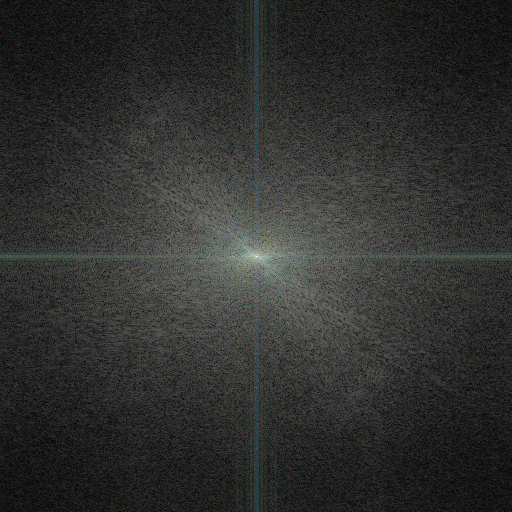
\includegraphics[scale=0.3]{img/lenac_fourier_phase.png}
  \label{fig.lenac_fourier_phase}
 }
 \subfigure[Widmo mocy przekształcenia Fouriera obrazka \textbf{lenac.bmp} (\ref{fig.lenac})]{
  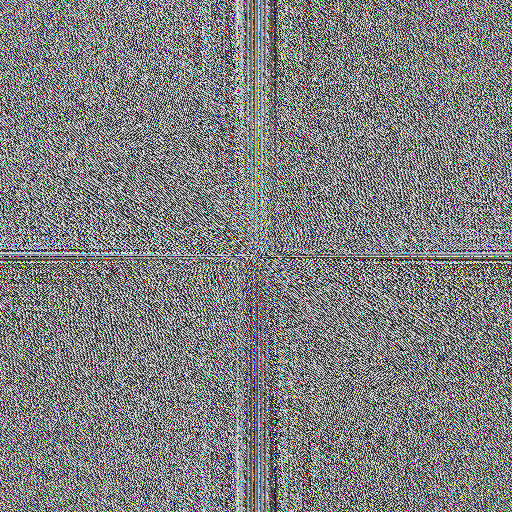
\includegraphics[scale=0.3]{img/lenac_fourier_magnitude.png}
  \label{fig.lenac_fourier_magnitude}
 }
 \subfigure[Widmo przekształcenia kosinusowego obrazka \textbf{lenac.bmp} (\ref{fig.lenac})]{
  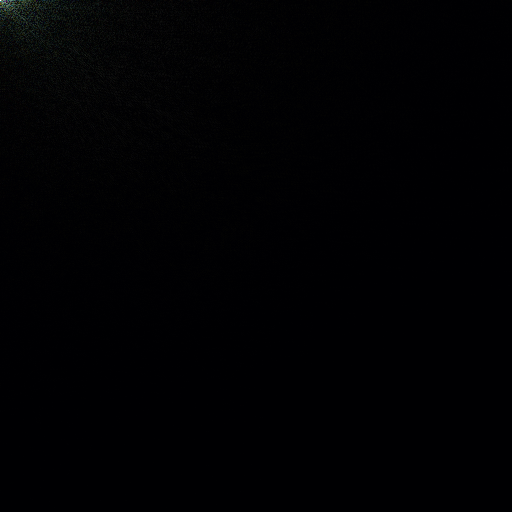
\includegraphics[scale=0.3]{img/lenac_cosine_phase.png}
  \label{fig.lenac_cosine_phase}
 }
\caption{Przekształcenia \textbf{lenac.bmp}}
\end{figure}

\begin{figure}
 \subfigure[Widmo fazy przekształcenia Fouriera obrazka \textbf{lena.bmp} (\ref{fig.lena})]{
  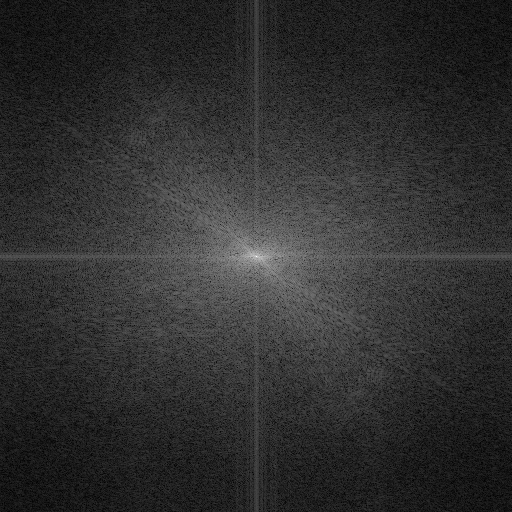
\includegraphics[scale=0.3]{img/lena_fourier_phase.png}
  \label{fig.lena_fourier_phase}
 }
 \subfigure[Widmo mocy przekształcenia Fouriera obrazka \textbf{lena.bmp} (\ref{fig.lena})]{
  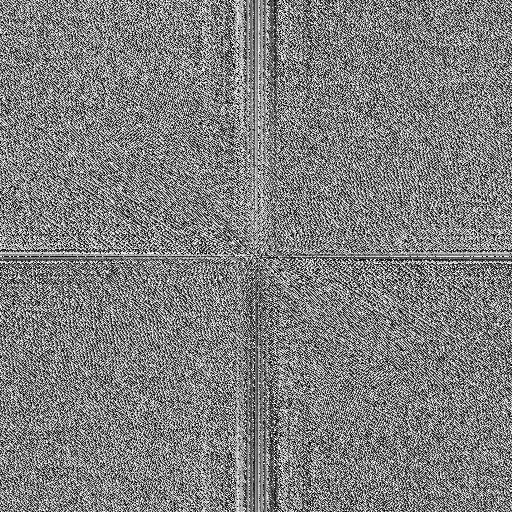
\includegraphics[scale=0.3]{img/lena_fourier_magnitude.png}
  \label{fig.lena_fourier_magnitude}
 }
 \subfigure[Widmo przekształcenia kosinusowego obrazka \textbf{lena.bmp} (\ref{fig.lena})]{
  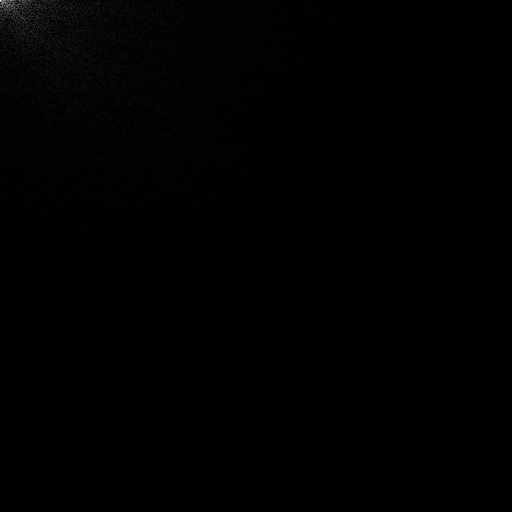
\includegraphics[scale=0.3]{img/lena_cosine_phase.png}
  \label{fig.lena_cosine_phase}
 }
\caption{Przekształcenia \textbf{lena.bmp}}
\end{figure}

\subsection{Filtracja dolnoprzepustowa}
Obrazki \ref{fig.lena_fourier_lowpass}, \ref{fig.lenac_fourier_lowpass}, \ref{fig.lena_cosine_lowpass} i \ref{fig.lenac_cosine_lowpass} przedstawiają wyniki filtrowania dolnoprzepustowego.

% fourier lowpass bw
\begin{figure}
 \subfigure[Obrazek \textbf{lena.bmp} (\ref{fig.lena}) po przekształceniu Fouriera i filtracji dolnoprzepustowej z parametrem $0.2R$]{
  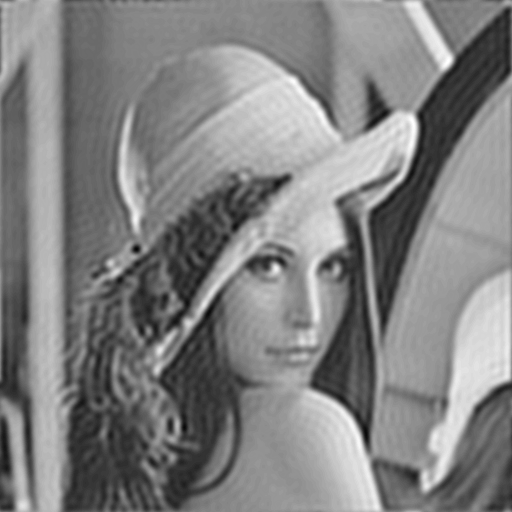
\includegraphics[scale=0.3]{img/lena_fourier_lowpass_0_2.png}
  \label{fig.lena_fourier_lowpass_0_2}
 }
 \subfigure[Obrazek \textbf{lena.bmp} (\ref{fig.lena}) po przekształceniu Fouriera i filtracji dolnoprzepustowej z parametrem $0.5R$]{
  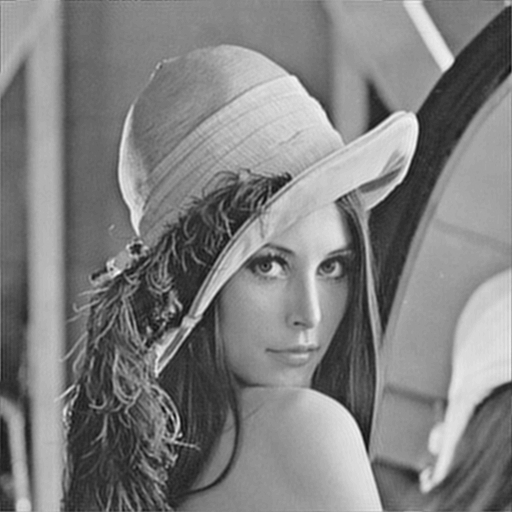
\includegraphics[scale=0.3]{img/lena_fourier_lowpass_0_5.png}
  \label{fig.lena_fourier_lowpass_0_5}
 }
 \subfigure[Obrazek \textbf{lena.bmp} (\ref{fig.lena}) po przekształceniu Fouriera i filtracji dolnoprzepustowej z parametrem $0.7R$]{
  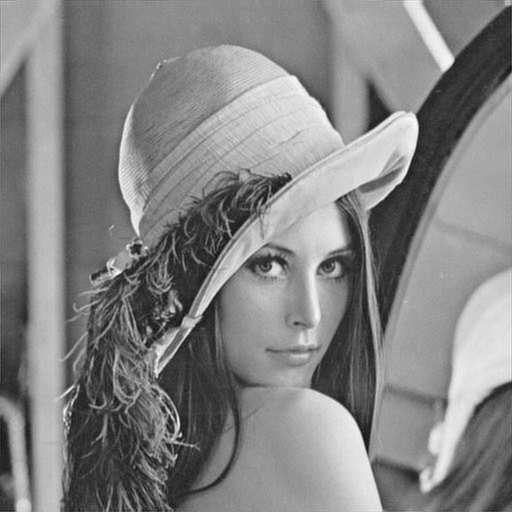
\includegraphics[scale=0.3]{img/lena_fourier_lowpass_0_7.png}
  \label{fig.lena_fourier_lowpass_0_7}
 }
\caption{Filtracja \textbf{lena.bmp} (Fourier)}
\label{fig.lena_fourier_lowpass}
\end{figure}

% fourier lowpass color
\begin{figure}
 \subfigure[Obrazek \textbf{lenac.bmp} (\ref{fig.lenac}) po przekształceniu Fouriera i filtracji dolnoprzepustowej z parametrem $0.2R$]{
  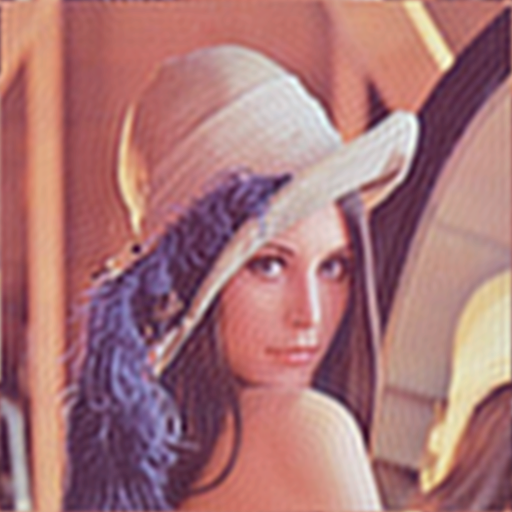
\includegraphics[scale=0.3]{img/lenac_fourier_lowpass_0_2.png}
  \label{fig.lenac_fourier_lowpass_0_2}
 }
 \subfigure[Obrazek \textbf{lenac.bmp} (\ref{fig.lenac}) po przekształceniu Fouriera i filtracji dolnoprzepustowej z parametrem $0.5R$]{
  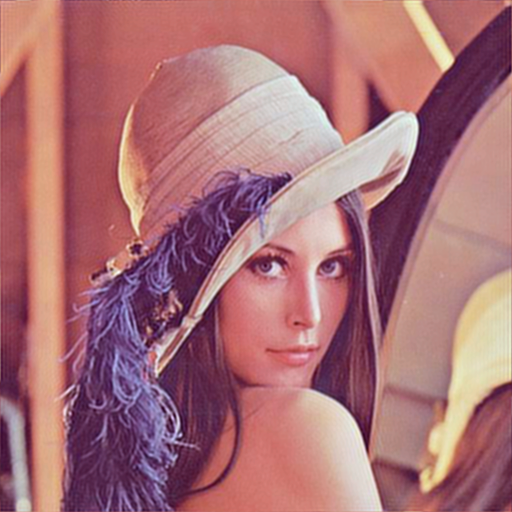
\includegraphics[scale=0.3]{img/lenac_fourier_lowpass_0_5.png}
  \label{fig.lenac_fourier_lowpass_0_5}
 }
 \subfigure[Obrazek \textbf{lenac.bmp} (\ref{fig.lenac}) po przekształceniu Fouriera i filtracji dolnoprzepustowej z parametrem $0.7R$]{
  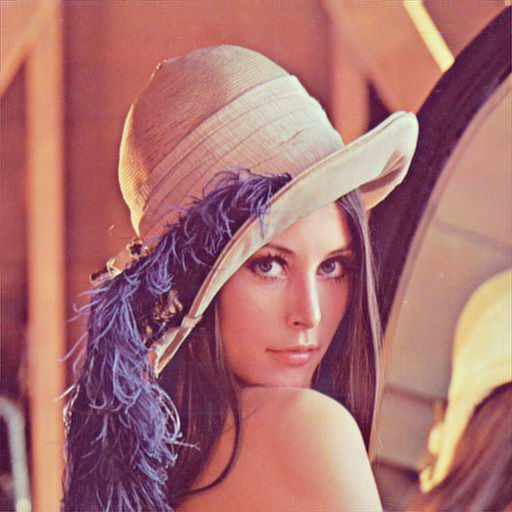
\includegraphics[scale=0.3]{img/lenac_fourier_lowpass_0_7.png}
  \label{fig.lenac_fourier_lowpass_0_7}
 }
\caption{Filtracja \textbf{lenac.bmp} (Fourier)}
\label{fig.lenac_fourier_lowpass}
\end{figure}

% cosine lowpass bw
\begin{figure}
 \subfigure[Obrazek \textbf{lena.bmp} (\ref{fig.lena}) po przekształceniu kosinusowym i filtracji dolnoprzepustowej z parametrem $0.2R$]{
  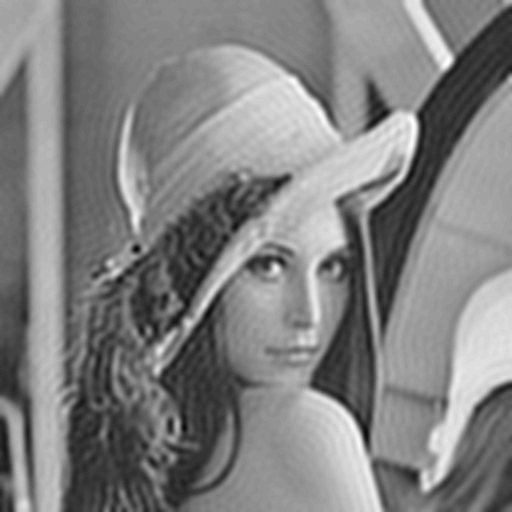
\includegraphics[scale=0.3]{img/lena_cosine_lowpass_0_2.png}
  \label{fig.lena_cosine_lowpass_0_2}
 }
 \subfigure[Obrazek \textbf{lena.bmp} (\ref{fig.lena}) po przekształceniu kosinusowym i filtracji dolnoprzepustowej z parametrem $0.5R$]{
  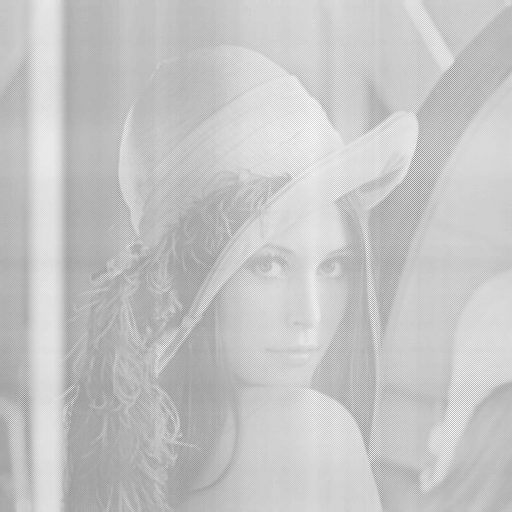
\includegraphics[scale=0.3]{img/lena_cosine_lowpass_0_5.png}
  \label{fig.lena_cosine_lowpass_0_5}
 }
 \subfigure[Obrazek \textbf{lena.bmp} (\ref{fig.lena}) po przekształceniu kosinusowym i filtracji dolnoprzepustowej z parametrem $0.7R$]{
  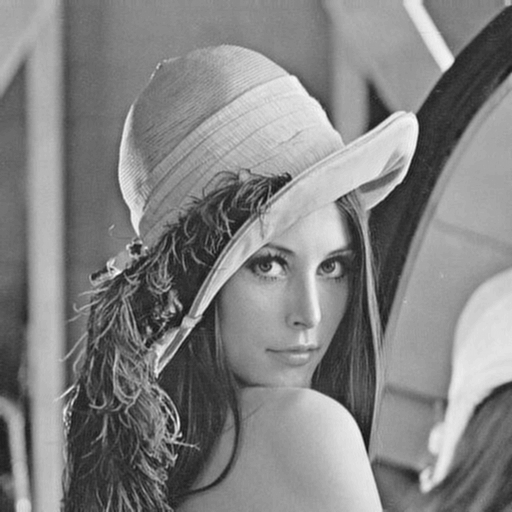
\includegraphics[scale=0.3]{img/lena_cosine_lowpass_0_7.png}
  \label{fig.lena_cosine_lowpass_0_7}
 }
\caption{Filtracja \textbf{lena.bmp} (kosinusowe)}
\label{fig.lena_cosine_lowpass}
\end{figure}

% cosine lowpass color
\begin{figure}
 \subfigure[Obrazek \textbf{lenac.bmp} (\ref{fig.lenac}) po przekształceniu kosinusowym i filtracji dolnoprzepustowej z parametrem $0.2R$]{
  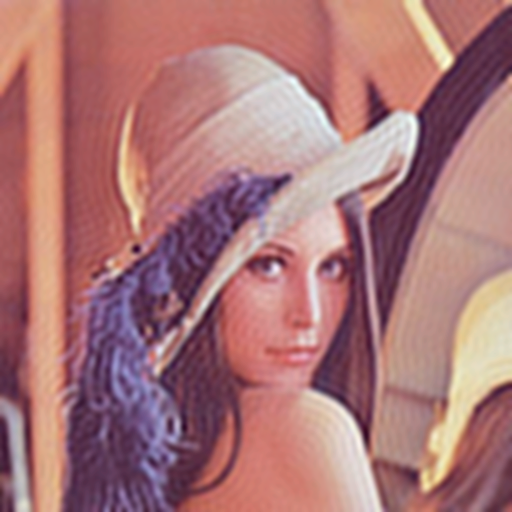
\includegraphics[scale=0.3]{img/lenac_cosine_lowpass_0_2.png}
  \label{fig.lenac_cosine_lowpass_0_2}
 }
 \subfigure[Obrazek \textbf{lenac.bmp} (\ref{fig.lenac}) po przekształceniu kosinusowym i filtracji dolnoprzepustowej z parametrem $0.5R$]{
  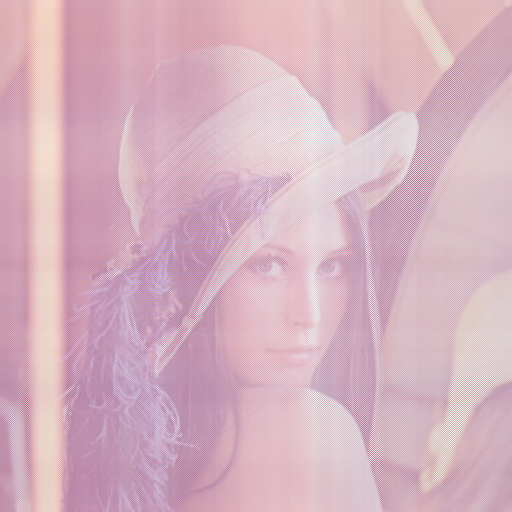
\includegraphics[scale=0.3]{img/lenac_cosine_lowpass_0_5.png}
  \label{fig.lenac_cosine_lowpass_0_5}
 }
 \subfigure[Obrazek \textbf{lenac.bmp} (\ref{fig.lenac}) po przekształceniu kosinusowym i filtracji dolnoprzepustowej z parametrem $0.7R$]{
  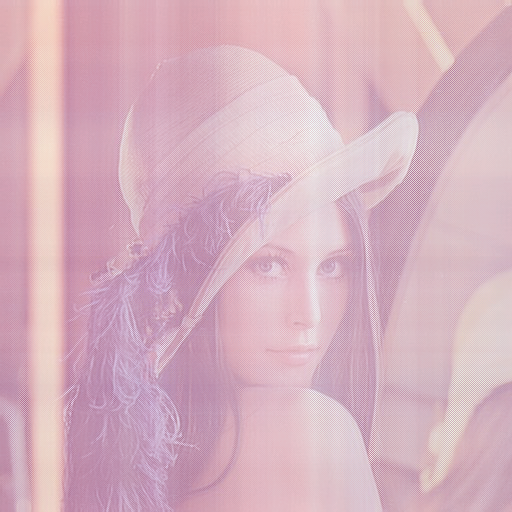
\includegraphics[scale=0.3]{img/lenac_cosine_lowpass_0_7.png}
  \label{fig.lenac_cosine_lowpass_0_7}
 }
\caption{Filtracja \textbf{lenac.bmp} (kosinusowe)}
\label{fig.lenac_cosine_lowpass}
\end{figure}

\subsection{Filtracja górnoprzepustowa}
Obrazki \ref{fig.lena_fourier_highpass}, \ref{fig.lenac_fourier_highpass}, \ref{fig.lena_cosine_highpass} i \ref{fig.lenac_cosine_highpass} przedstawiają wyniki filtrowania górnoprzepustowego.

% fourier highpass bw
\begin{figure}
 \subfigure[Obrazek \textbf{lena.bmp} (\ref{fig.lena}) po przekształceniu Fouriera i filtracji górnoprzepustowej z parametrem $0.2R$]{
  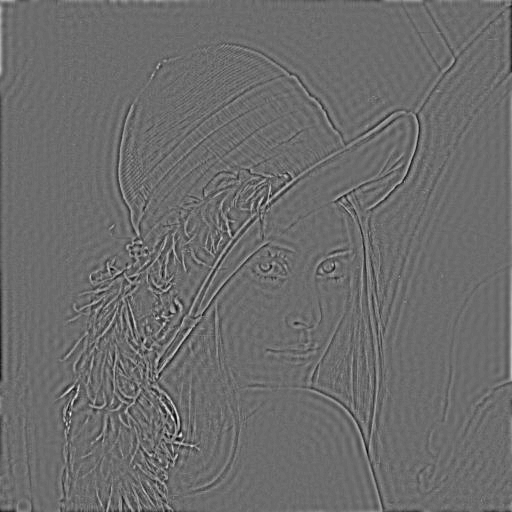
\includegraphics[scale=0.3]{img/lena_fourier_highpass_0_2.png}
  \label{fig.lena_fourier_highpass_0_2}
 }
 \subfigure[Obrazek \textbf{lena.bmp} (\ref{fig.lena}) po przekształceniu Fouriera i filtracji górnoprzepustowej z parametrem $0.5R$]{
  
\includegraphics[scale=0.3]{img/lena_fourier_highpass_0_5.png}
  \label{fig.lena_fourier_highpass_0_5}
 }
 \subfigure[Obrazek \textbf{lena.bmp} (\ref{fig.lena}) po przekształceniu Fouriera i filtracji górnoprzepustowej z parametrem $0.7R$]{
  
\includegraphics[scale=0.3]{img/lena_fourier_highpass_0_7.png}
  \label{fig.lena_fourier_highpass_0_7}
 }
\caption{Filtracja \textbf{lena.bmp} (Fourier)}
\label{fig.lena_fourier_highpass}
\end{figure}

% fourier highpass color
\begin{figure}
 \subfigure[Obrazek \textbf{lenac.bmp} (\ref{fig.lenac}) po przekształceniu Fouriera i filtracji górnoprzepustowej z parametrem $0.2R$]{
  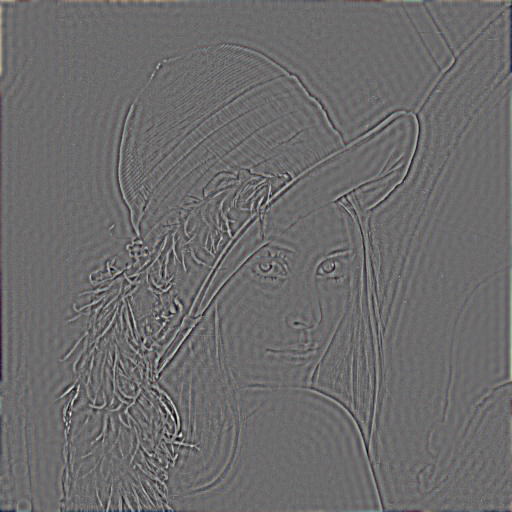
\includegraphics[scale=0.3]{img/lenac_fourier_highpass_0_2.png}
  \label{fig.lenac_fourier_highpass_0_2}
 }
 \subfigure[Obrazek \textbf{lenac.bmp} (\ref{fig.lenac}) po przekształceniu Fouriera i filtracji górnoprzepustowej z parametrem $0.5R$]{
  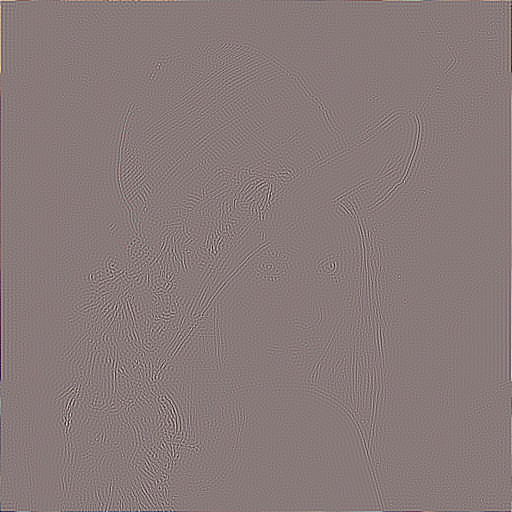
\includegraphics[scale=0.3]{img/lenac_fourier_highpass_0_5.png}
  \label{fig.lenac_fourier_highpass_0_5}
 }
 \subfigure[Obrazek \textbf{lenac.bmp} (\ref{fig.lenac}) po przekształceniu Fouriera i filtracji górnoprzepustowej z parametrem $0.7R$]{
  
\includegraphics[scale=0.3]{img/lenac_fourier_highpass_0_7.png}
  \label{fig.lenac_fourier_highpass_0_7}
 }
\caption{Filtracja \textbf{lenac.bmp} (Fourier)}
\label{fig.lenac_fourier_highpass}
\end{figure}

% cosine highpass bw
\begin{figure}
 \subfigure[Obrazek \textbf{lena.bmp} (\ref{fig.lena}) po przekształceniu kosinusowym i filtracji górnoprzepustowej z parametrem $0.2R$]{
  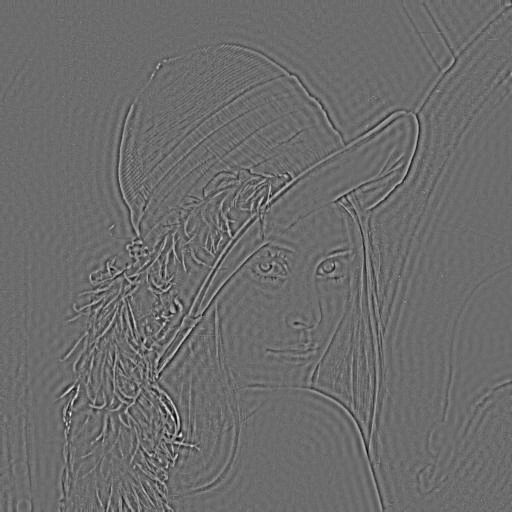
\includegraphics[scale=0.3]{img/lena_cosine_highpass_0_2.png}
  \label{fig.lena_cosine_highpass_0_2}
 }
 \subfigure[Obrazek \textbf{lena.bmp} (\ref{fig.lena}) po przekształceniu kosinusowym i filtracji górnoprzepustowej z parametrem $0.5R$]{
  
\includegraphics[scale=0.3]{img/lena_cosine_highpass_0_5.png}
  \label{fig.lena_cosine_highpass_0_5}
 }
 \subfigure[Obrazek \textbf{lena.bmp} (\ref{fig.lena}) po przekształceniu kosinusowym i filtracji górnoprzepustowej z parametrem $0.7R$]{
  
\includegraphics[scale=0.3]{img/lena_cosine_highpass_0_7.png}
  \label{fig.lena_cosine_highpass_0_7}
 }
\caption{Filtracja \textbf{lena.bmp} (kosinusowe)}
\label{fig.lena_cosine_highpass}
\end{figure}

% cosine highpass color
\begin{figure}
 \subfigure[Obrazek \textbf{lenac.bmp} (\ref{fig.lenac}) po przekształceniu kosinusowym i filtracji górnoprzepustowej z parametrem $0.2R$]{
  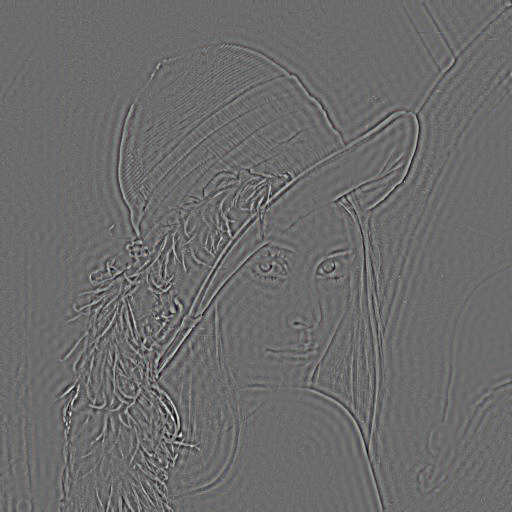
\includegraphics[scale=0.3]{img/lenac_cosine_highpass_0_2.png}
  \label{fig.lenac_cosine_highpass_0_2}
 }
 \subfigure[Obrazek \textbf{lenac.bmp} (\ref{fig.lenac}) po przekształceniu kosinusowym i filtracji górnoprzepustowej z parametrem $0.5R$]{
  
\includegraphics[scale=0.3]{img/lenac_cosine_highpass_0_5.png}
  \label{fig.lenac_cosine_highpass_0_5}
 }
 \subfigure[Obrazek \textbf{lenac.bmp} (\ref{fig.lenac}) po przekształceniu kosinusowym i filtracji górnoprzepustowej z parametrem $0.7R$]{
  
\includegraphics[scale=0.3]{img/lenac_cosine_highpass_0_7.png}
  \label{fig.lenac_cosine_highpass_0_7}
 }
\caption{Filtracja \textbf{lenac.bmp} (kosinusowe)}
\label{fig.lenac_cosine_highpass}
\end{figure}

\subsection{Filtracja pasmowoprzepustowa}
Obrazki \ref{fig.lena_fourier_bandpass}, \ref{fig.lenac_fourier_bandpass}, \ref{fig.lena_cosine_bandpass} i \ref{fig.lenac_cosine_bandpass} przedstawiają wyniki filtrowania pasmowoprzepustowego.

% fourier bandpass bw
\begin{figure}
 \subfigure[Obrazek \textbf{lena.bmp} (\ref{fig.lena}) po przekształceniu Fouriera i filtracji pasmowoprzepustowej z parametrami $0.1R$ i $0.9R$]{
  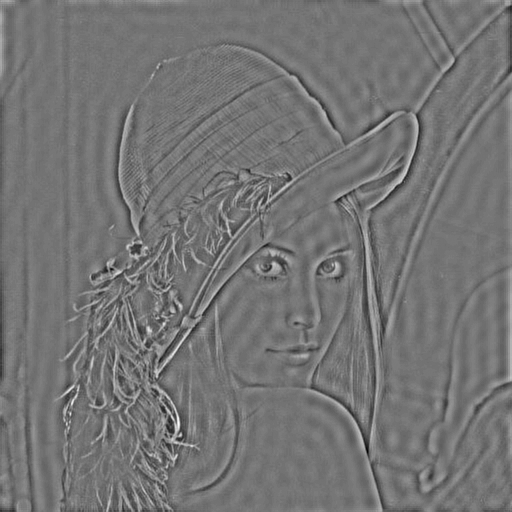
\includegraphics[scale=0.3]{img/lena_fourier_bandpass_0_1_0_9.png}
  \label{fig.lena_fourier_bandpass_0_1_0_9}
 }
 \subfigure[Obrazek \textbf{lena.bmp} (\ref{fig.lena}) po przekształceniu Fouriera i filtracji pasmowoprzepustowej z parametrami $0.2R$ i $0.8R$]{
  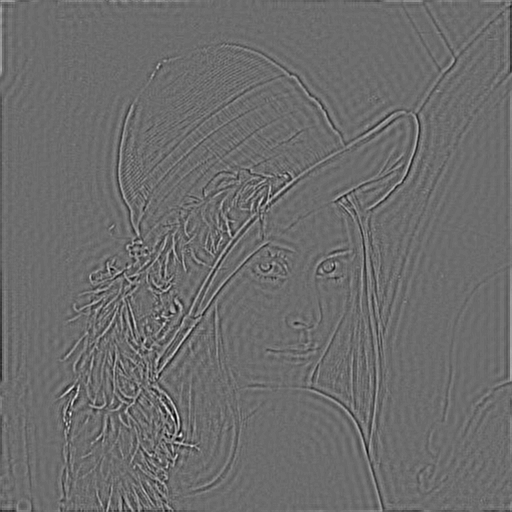
\includegraphics[scale=0.3]{img/lena_fourier_bandpass_0_2_0_8.png}
  \label{fig.lena_fourier_bandpass_0_2_0_8}
 }
 \subfigure[Obrazek \textbf{lena.bmp} (\ref{fig.lena}) po przekształceniu Fouriera i filtracji pasmowoprzepustowej z parametrami $0.4R$ i $0.6R$]{
  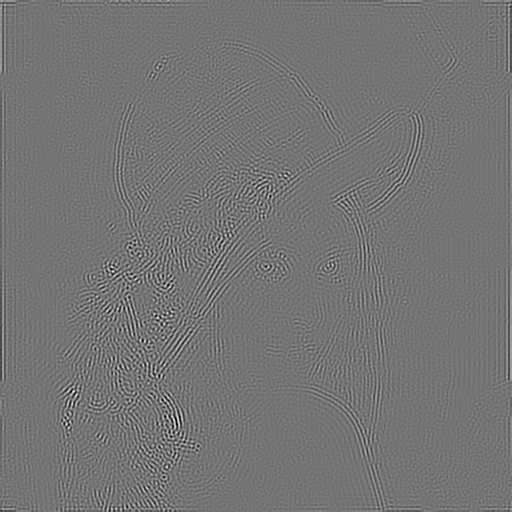
\includegraphics[scale=0.3]{img/lena_fourier_bandpass_0_4_0_6.png}
  \label{fig.lena_fourier_bandpass_0_4_0_6}
 }
\caption{Filtracja \textbf{lena.bmp} (Fourier)}
\label{fig.lena_fourier_bandpass}
\end{figure}

% fourier bandpass color
\begin{figure}
 \subfigure[Obrazek \textbf{lenac.bmp} (\ref{fig.lenac}) po przekształceniu Fouriera i filtracji pasmowoprzepustowej z parametrami $0.1R$ i $0.9R$]{
  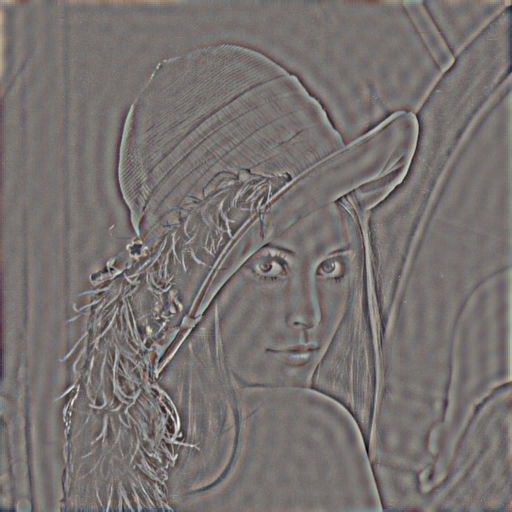
\includegraphics[scale=0.3]{img/lenac_fourier_bandpass_0_1_0_9.png}
  \label{fig.lenac_fourier_bandpass_0_1_0_9}
 }
 \subfigure[Obrazek \textbf{lenac.bmp} (\ref{fig.lenac}) po przekształceniu Fouriera i filtracji pasmowoprzepustowej z parametrami $0.2R$ i $0.8R$]{
  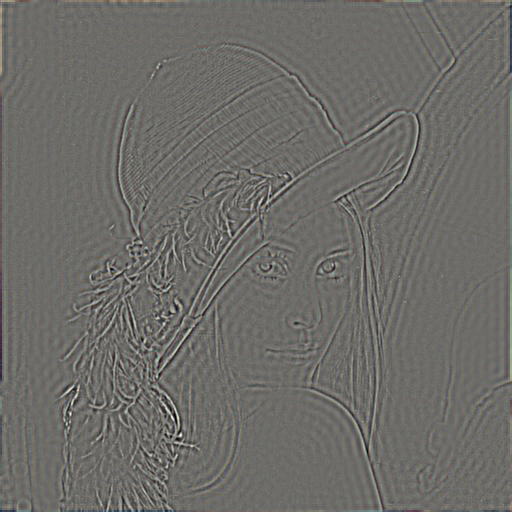
\includegraphics[scale=0.3]{img/lenac_fourier_bandpass_0_2_0_8.png}
  \label{fig.lenac_fourier_bandpass_0_2_0_8}
 }
 \subfigure[Obrazek \textbf{lenac.bmp} (\ref{fig.lenac}) po przekształceniu Fouriera i filtracji pasmowoprzepustowej z parametrami $0.4R$ i $0.6R$]{
  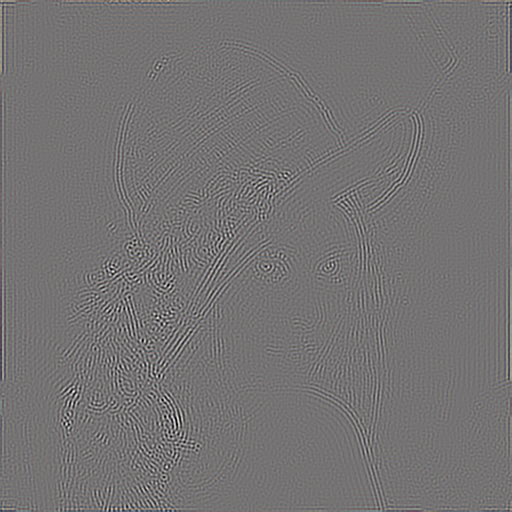
\includegraphics[scale=0.3]{img/lenac_fourier_bandpass_0_4_0_6.png}
  \label{fig.lenac_fourier_bandpass_0_4_0_6}
 }
\caption{Filtracja \textbf{lenac.bmp} (Fourier)}
\label{fig.lenac_fourier_bandpass}
\end{figure}

% cosine bandpass bw
\begin{figure}
 \subfigure[Obrazek \textbf{lena.bmp} (\ref{fig.lena}) po przekształceniu kosinusowym i filtracji pasmowoprzepustowej z parametrami $0.1R$ i $0.9R$]{
  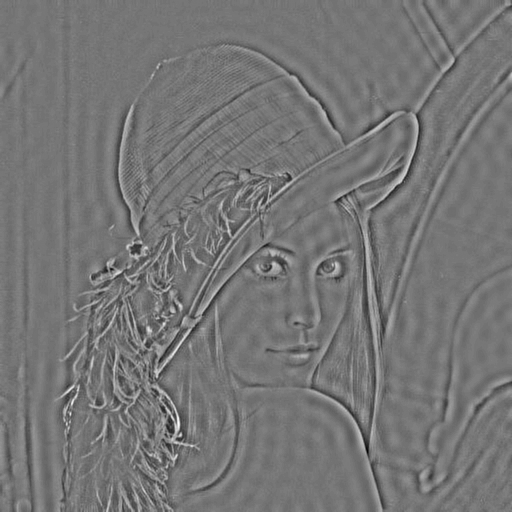
\includegraphics[scale=0.3]{img/lena_cosine_bandpass_0_1_0_9.png}
  \label{fig.lena_cosine_bandpass_0_1_0_9}
 }
 \subfigure[Obrazek \textbf{lena.bmp} (\ref{fig.lena}) po przekształceniu kosinusowym i filtracji pasmowoprzepustowej z parametrami $0.1R$ i $0.9R$]{
  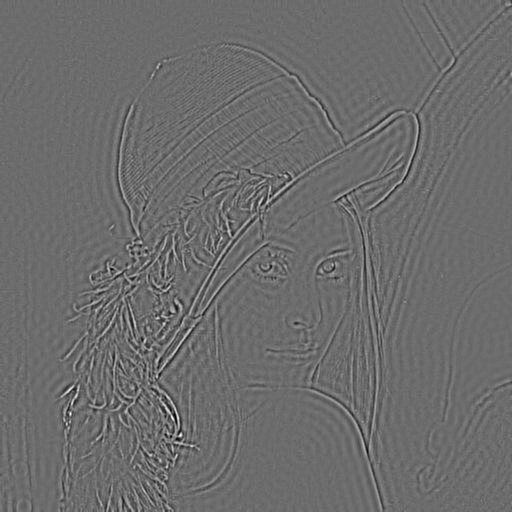
\includegraphics[scale=0.3]{img/lena_cosine_bandpass_0_2_0_8.png}
  \label{fig.lena_cosine_bandpass_0_2_0_8}
 }
 \subfigure[Obrazek \textbf{lena.bmp} (\ref{fig.lena}) po przekształceniu kosinusowym i filtracji pasmowoprzepustowej z parametrami $0.1R$ i $0.9R$]{
  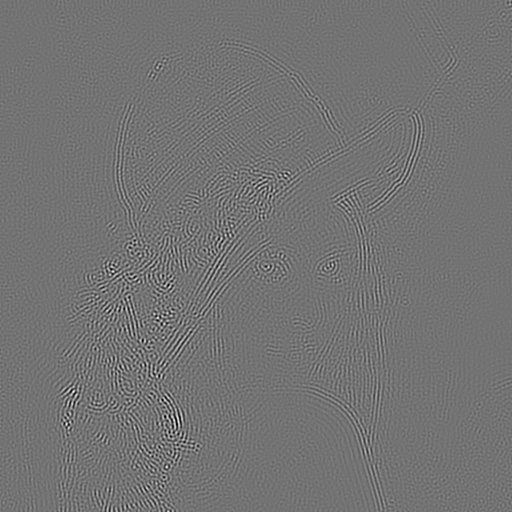
\includegraphics[scale=0.3]{img/lena_cosine_bandpass_0_4_0_6.png}
  \label{fig.lena_cosine_bandpass_0_4_0_6}
 }
\caption{Filtracja \textbf{lena.bmp} (kosinusowe)}
\label{fig.lena_cosine_bandpass}
\end{figure}

% cosine bandpass color
\begin{figure}
 \subfigure[Obrazek \textbf{lenac.bmp} (\ref{fig.lenac}) po przekształceniu kosinusowym i filtracji pasmowoprzepustowej z parametrami $0.1R$ i $0.9R$]{
  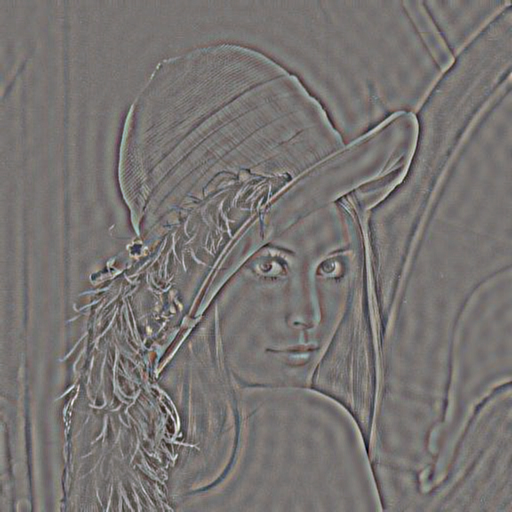
\includegraphics[scale=0.3]{img/lenac_cosine_bandpass_0_1_0_9.png}
  \label{fig.lenac_cosine_bandpass_0_1_0_9}
 }
 \subfigure[Obrazek \textbf{lenac.bmp} (\ref{fig.lenac}) po przekształceniu kosinusowym i filtracji pasmowoprzepustowej z parametrami $0.1R$ i $0.9R$]{
  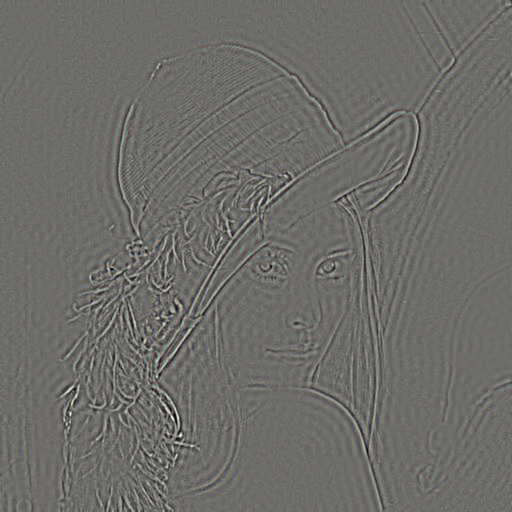
\includegraphics[scale=0.3]{img/lenac_cosine_bandpass_0_2_0_8.png}
  \label{fig.lenac_cosine_bandpass_0_2_0_8}
 }
 \subfigure[Obrazek \textbf{lenac.bmp} (\ref{fig.lenac}) po przekształceniu kosinusowym i filtracji pasmowoprzepustowej z parametrami $0.1R$ i $0.9R$]{
  
\includegraphics[scale=0.3]{img/lenac_cosine_bandpass_0_4_0_6.png}
  \label{fig.lenac_cosine_bandpass_0_4_0_6}
 }
\caption{Filtracja \textbf{lenac.bmp} (kosinusowe)}
\label{fig.lenac_cosine_bandpass}
\end{figure}

\subsection{Filtracja pasmowozaporowa}
Obrazki \ref{fig.lena_fourier_bandstop}, \ref{fig.lenac_fourier_bandstop}, \ref{fig.lena_cosine_bandstop} i \ref{fig.lenac_cosine_bandstop} przedstawiają wyniki filtrowania pasmowozaporowego.

% fourier bandstop bw
\begin{figure}
 \subfigure[Obrazek \textbf{lena.bmp} (\ref{fig.lena}) po przekształceniu Fouriera i filtracji pasmowozaporowej z parametrami $0.1R$ i $0.9R$]{
  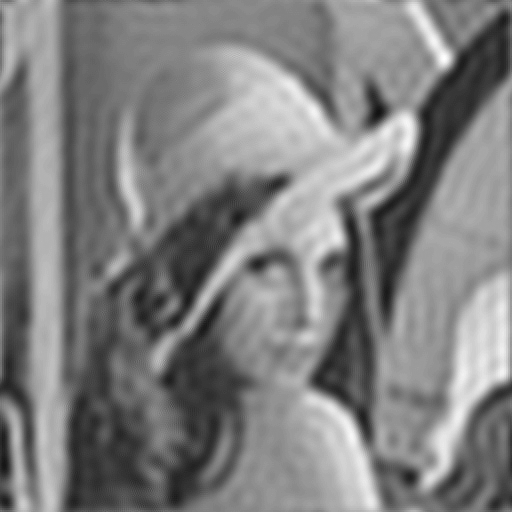
\includegraphics[scale=0.3]{img/lena_fourier_bandstop_0_1_0_9.png}
  \label{fig.lena_fourier_bandstop_0_1_0_9}
 }
 \subfigure[Obrazek \textbf{lena.bmp} (\ref{fig.lena}) po przekształceniu Fouriera i filtracji pasmowozaporowej z parametrami $0.2R$ i $0.8R$]{
  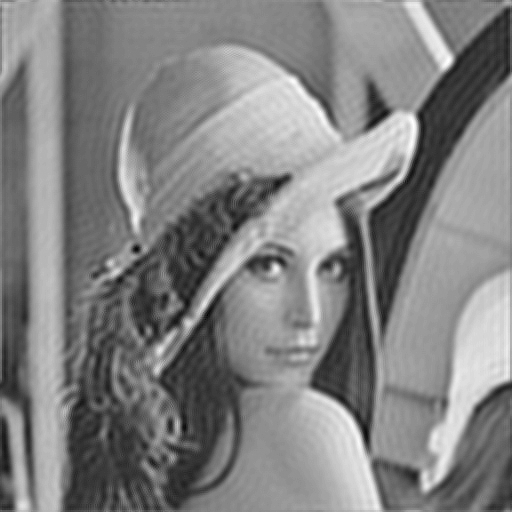
\includegraphics[scale=0.3]{img/lena_fourier_bandstop_0_2_0_8.png}
  \label{fig.lena_fourier_bandstop_0_2_0_8}
 }
 \subfigure[Obrazek \textbf{lena.bmp} (\ref{fig.lena}) po przekształceniu Fouriera i filtracji pasmowozaporowej z parametrami $0.4R$ i $0.6R$]{
  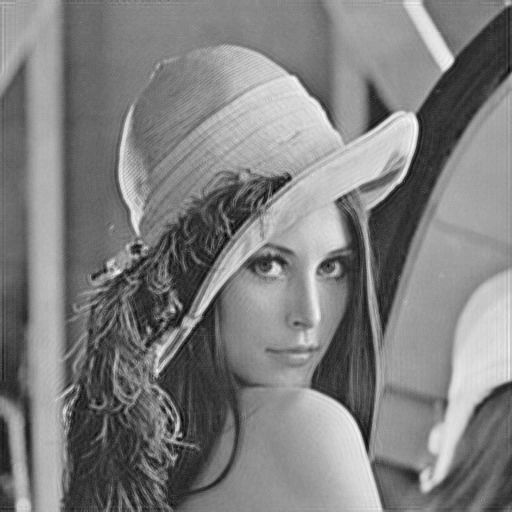
\includegraphics[scale=0.3]{img/lena_fourier_bandstop_0_4_0_6.png}
  \label{fig.lena_fourier_bandstop_0_4_0_6}
 }
\caption{Filtracja \textbf{lena.bmp} (Fourier)}
\label{fig.lena_fourier_bandstop}
\end{figure}

% fourier bandstop color
\begin{figure}
 \subfigure[Obrazek \textbf{lenac.bmp} (\ref{fig.lenac}) po przekształceniu Fouriera i filtracji pasmowozaporowej z parametrami $0.1R$ i $0.9R$]{
  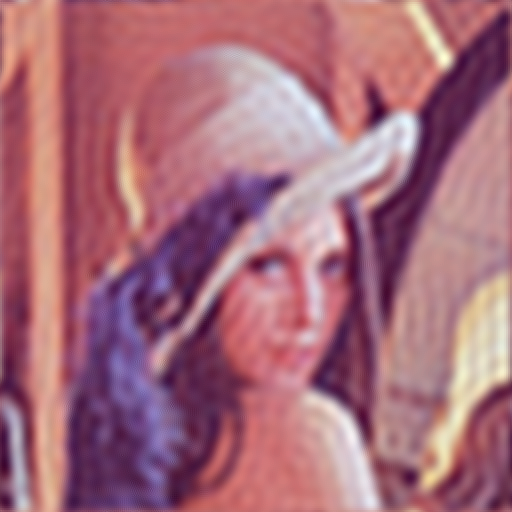
\includegraphics[scale=0.3]{img/lenac_fourier_bandstop_0_1_0_9.png}
  \label{fig.lenac_fourier_bandstop_0_1_0_9}
 }
 \subfigure[Obrazek \textbf{lenac.bmp} (\ref{fig.lenac}) po przekształceniu Fouriera i filtracji pasmowozaporowej z parametrami $0.2R$ i $0.8R$]{
  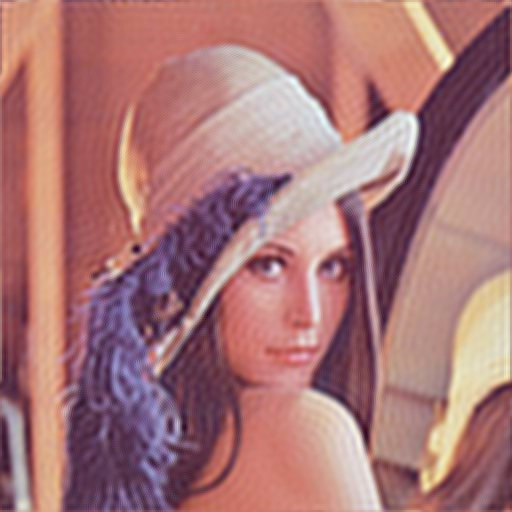
\includegraphics[scale=0.3]{img/lenac_fourier_bandstop_0_2_0_8.png}
  \label{fig.lenac_fourier_bandstop_0_2_0_8}
 }
 \subfigure[Obrazek \textbf{lenac.bmp} (\ref{fig.lenac}) po przekształceniu Fouriera i filtracji pasmowozaporowej z parametrami $0.4R$ i $0.6R$]{
  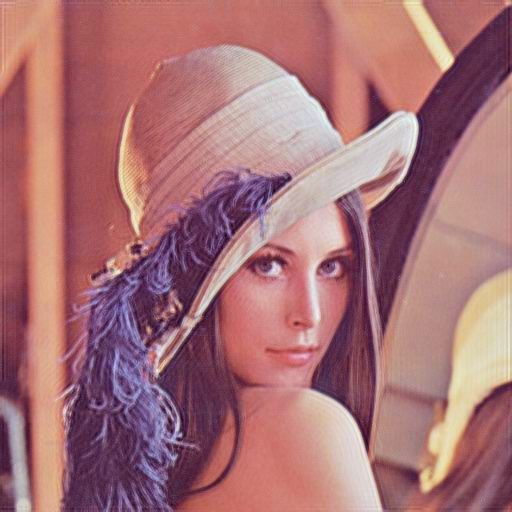
\includegraphics[scale=0.3]{img/lenac_fourier_bandstop_0_4_0_6.png}
  \label{fig.lenac_fourier_bandstop_0_4_0_6}
 }
\caption{Filtracja \textbf{lenac.bmp} (Fourier)}
\label{fig.lenac_fourier_bandstop}
\end{figure}

% cosine bandstop bw
\begin{figure}
 \subfigure[Obrazek \textbf{lena.bmp} (\ref{fig.lena}) po przekształceniu kosinusowym i filtracji pasmowozaporowej z parametrami $0.1R$ i $0.9R$]{
  \includegraphics[scale=0.3]{img/lena_cosine_bandstop_0_1_0_9.png}
  \label{fig.lena_cosine_bandstop_0_1_0_9}
 }
 \subfigure[Obrazek \textbf{lena.bmp} (\ref{fig.lena}) po przekształceniu kosinusowym i filtracji pasmowozaporowej z parametrami $0.1R$ i $0.9R$]{
  \includegraphics[scale=0.3]{img/lena_cosine_bandstop_0_2_0_8.png}
  \label{fig.lena_cosine_bandstop_0_2_0_8}
 }
 \subfigure[Obrazek \textbf{lena.bmp} (\ref{fig.lena}) po przekształceniu kosinusowym i filtracji pasmowozaporowej z parametrami $0.1R$ i $0.9R$]{
  \includegraphics[scale=0.3]{img/lena_cosine_bandstop_0_4_0_6.png}
  \label{fig.lena_cosine_bandstop_0_4_0_6}
 }
\caption{Filtracja \textbf{lena.bmp} (kosinusowe)}
\label{fig.lena_cosine_bandstop}
\end{figure}

% cosine bandstop color
\begin{figure}
 \subfigure[Obrazek \textbf{lenac.bmp} (\ref{fig.lenac}) po przekształceniu kosinusowym i filtracji pasmowozaporowej z parametrami $0.1R$ i $0.9R$]{
  \includegraphics[scale=0.3]{img/lenac_cosine_bandstop_0_1_0_9.png}
  \label{fig.lenac_cosine_bandstop_0_1_0_9}
 }
 \subfigure[Obrazek \textbf{lenac.bmp} (\ref{fig.lenac}) po przekształceniu kosinusowym i filtracji pasmowozaporowej z parametrami $0.1R$ i $0.9R$]{
  \includegraphics[scale=0.3]{img/lenac_cosine_bandstop_0_2_0_8.png}
  \label{fig.lenac_cosine_bandstop_0_2_0_8}
 }
 \subfigure[Obrazek \textbf{lenac.bmp} (\ref{fig.lenac}) po przekształceniu kosinusowym i filtracji pasmowozaporowej z parametrami $0.1R$ i $0.9R$]{
  \includegraphics[scale=0.3]{img/lenac_cosine_bandstop_0_4_0_6.png}
  \label{fig.lenac_cosine_bandstop_0_4_0_6}
 }
\caption{Filtracja \textbf{lenac.bmp} (kosinusowe)}
\label{fig.lenac_cosine_bandstop}
\end{figure}

\subsection{Przesunięcie fazowe}
Obrazki \ref{fig.lenac_fourier_phaseshift} przedstawiają wynik przesunięcia fazowego widm przekształcenia Fouriera.

\begin{figure}
 \subfigure[Obrazek \textbf{lenac.bmp} (\ref{fig.lenac}) po przekształceniu Fouriera i przesunięciu widm w fazie o $8, 8$]{
  \includegraphics[scale=0.5]{img/lenac_fourier_phaseshift_8_8.png}
  \label{fig.lenac_fourier_phaseshift_8_8}
 }
 \subfigure[Obrazek \textbf{lenac.bmp} (\ref{fig.lenac}) po przekształceniu Fouriera i przesunięciu widm w fazie o $-8, -8$]{
  \includegraphics[scale=0.5]{img/lenac_fourier_phaseshift_-8_-8.png}
  \label{fig.lenac_fourier_phaseshift_-8_-8}
 }
\caption{Przesunięcie fazowe widm \textbf{lenac.bmp}}
\label{fig.lenac_fourier_phaseshift}
\end{figure}

\section{Dyskusja}
Podczas obróbki obrazów najbardziej charakterystyczną cechą jest fakt, że największy udział mają składowe o niskich częstotliwościach. Tyczy się to zarówno przekształcenia Fouriera jak i kosinusowego. Usunięcie tych składowych, np. filtrem górnoprzepustowym, powoduje znaczne pogorszenie jakości obrazu. Dla odmiany filtracja górnoprzepustowa, w zależności od zadanego promienia, wprowadza bardzo mało zauważalne zmiany w obrazie. Właściwości tej cechy powodują, że można ją wykorzystać do stratnej kompresji obrazu. W praktyce kompresja JPEG opiera się o DCT, gdzie obraz dzielony jest na fragmenty wielkości 8x8 pikseli, wykoywane jest DCT, a elementy bliskie zeru są zerowane. Podejście takie umożliwia wykorzystanie wartości DCT znanych zawczasu \ppauza nie potrzeba ich zapisywać w pliku i posiada dodatkową przewagę nad ,,jednym dużym DCT'', którą jest możliwość wystąpienia powtórzeń bloków, co dodatkowo pozwala zwiększyć stopień kompresji.

\begin{thebibliography}{9}
\bibitem{librow} Sergey Chernenko. \textit{Fast Fourier Transform \ppauza FFT} [online]. Dostęp: 14.05.2011. Dostępny w Internecie: \url{http://www.librow.com/articles/article-10}
\bibitem{tr802} Syed Ali Khayam. \textit{The Discrete Cosine Transform (DCT): Theory and Application} [online]. Dostęp: 14.05.2011. Dostępny w Internecie: \url{http://www.wisnet.seecs.edu.pk/publications/tech_reports/DCT_TR802.pdf}
\bibitem{e186} Ruye Wang. \textit{Discrete Cosine Transform \ppauza E186 handout} [online]. Dostęp: 14.05.2011. Dostępny w Internecie: \url{http://www.wisnet.seecs.edu.pk/publications/tech_reports/DCT_TR802.pdf}
\end{thebibliography}


\end{document}